\documentclass[conference]{IEEEtran}

\usepackage{amsmath,amssymb,amsfonts}
\usepackage{graphicx}
\usepackage{textcomp}
\usepackage{xcolor}
\usepackage{url}
\usepackage[hidelinks]{hyperref}
\usepackage{booktabs}
\usepackage{float}
\usepackage{listings}
\usepackage{subcaption}
\usepackage[newfloat]{minted}
\pagestyle{plain}

\setminted{
    fontsize=\scriptsize,
    breaklines=true,
    bgcolor=gray!8,
    frame=none,
    xleftmargin=6pt
}

\lstdefinestyle{code}{
    backgroundcolor=\color{gray!8},
    basicstyle=\ttfamily\scriptsize,
    keywordstyle=\color{green!45!black}\bfseries,
    commentstyle=\color{gray},
    stringstyle=\color{red!60!black},
    breaklines=true,
    breakatwhitespace=false,
    postbreak=\mbox{\textcolor{gray}{$\hookrightarrow$}\space},
    frame=none,
    numbers=none,
    showstringspaces=false,
    captionpos=b,
    columns=fullflexible,
    keepspaces=true,
    xleftmargin=8pt,
    framexleftmargin=8pt,
    aboveskip=6pt,
    belowskip=6pt
}
\lstset{style=code}

% Plain style for the file tree
\lstdefinestyle{plain}{
    backgroundcolor=\color{gray!8},
    basicstyle=\ttfamily\scriptsize,
    breaklines=true,
    frame=none,
    numbers=none,
    showstringspaces=false,
    xleftmargin=8pt,
    framexleftmargin=8pt,
    aboveskip=6pt,
    belowskip=6pt
}

\raggedbottom

% Each listing below is wrapped in word counter skip markers, so the code is
% not counted. Without them texcount reads the xacro snippets as maths.

\begin{document}

\title{ACIT4820: Assignment 3 \\[4pt] \normalsize \textit{Total words: }}

\author{
    \IEEEauthorblockN{Felix Boehm}
    HELLO THOMAS!!
    \IEEEauthorblockA{OsloMet \\ feboe8099@oslomet.no}
     \and
    \IEEEauthorblockN{Thomas Heim}
    \IEEEauthorblockA{OsloMet \\ thhei7342@oslomet.no}
}

\maketitle

\section{Method}
We used Felix quantum computer to finish the assignment!


\section{Results}

\subsection{Task 1}
We calculated the inertia for each link by hand. We took the shape and the size
from the collision tag, not from the mesh. All of our values landed inside the
$10^{-5}$ to $10^{-1}$\,kg\,m$^2$ range. Our wheel also came out at the same
numbers as the example in the assignment text. That told us the masses and the
dimensions were right.




\smallskip
\textbf{\texttt{base\_link}}, cylinder, \mbox{$r=0.16$}, \mbox{$h=0.06$},
\mbox{$m=5.0$\,kg}:
\begin{align*}
I_{xx}=I_{yy} &= \frac{1}{12}m(3r^2+h^2) \\
              &= \frac{1}{12}(5.0)(0.0804) \\
              &= 3.35\times10^{-2}~\mathrm{kg\,m^2} \\[4pt]
I_{zz}        &= \frac{1}{2}mr^2 \\
              &= \frac{1}{2}(5.0)(0.0256) \\
              &= 6.40\times10^{-2}~\mathrm{kg\,m^2}
\end{align*}

\smallskip
\textbf{\texttt{left\_wheel\_link}} and \textbf{\texttt{right\_wheel\_link}},
cylinder, \mbox{$r=0.03$}, \mbox{$w=0.025$}, \mbox{$m=0.2$\,kg} each:
\begin{align*}
I_{xx}=I_{yy} &= \frac{1}{12}m(3r^2+w^2) \\
              &= \frac{1}{12}(0.2)(0.003325) \\
              &= 5.54\times10^{-5}~\mathrm{kg\,m^2} \\[4pt]
I_{zz}        &= \frac{1}{2}mr^2 \\
              &= \frac{1}{2}(0.2)(0.0009) \\
              &= 9.00\times10^{-5}~\mathrm{kg\,m^2}
\end{align*}

\smallskip
\textbf{\texttt{caster\_wheel\_link}}, sphere, \mbox{$r=0.02$},
\mbox{$m=0.1$\,kg}:
\begin{align*}
I_{xx}=I_{yy}=I_{zz} &= \frac{2}{5}mr^2 \\
                     &= \frac{2}{5}(0.1)(0.0004) \\
                     &= 1.60\times10^{-5}~\mathrm{kg\,m^2}
\end{align*}

\smallskip
\textbf{\texttt{lidar\_link}}, cylinder, \mbox{$r=0.03$},
\mbox{$h=0.01$}, \mbox{$m=0.1$\,kg}:
\begin{align*}
I_{xx}=I_{yy} &= \frac{1}{12}m(3r^2+h^2) \\
              &= \frac{1}{12}(0.1)(0.0028) \\
              &= 2.33\times10^{-5}~\mathrm{kg\,m^2} \\[4pt]
I_{zz}        &= \frac{1}{2}mr^2 \\
              &= \frac{1}{2}(0.1)(0.0009) \\
              &= 4.50\times10^{-5}~\mathrm{kg\,m^2}
\end{align*}



Our wheel is turned by its joint, not inside the link. So in the wheel link's own frame the round axis is still $z$, and the symmetry term stays on $I_{zz}$. Had we rotated the geometry inside the link, it would have moved to $I_{yy}$.

The physics comes from the collision tags and not from the visuals, so we
checked them in RViz. We turned on Collision in the RobotModel display and
lowered the Alpha to 0.3. Figure~\ref{fig:t1_collision} shows the result. The
body cylinder sits inside the mesh and nothing is floating or offset. The wheel
cylinders stick out a little on each side. That is correct, because the wheel
mesh is thinner than the $0.025$\,m we used for the collision.

\begin{figure}[H]
    \centering
    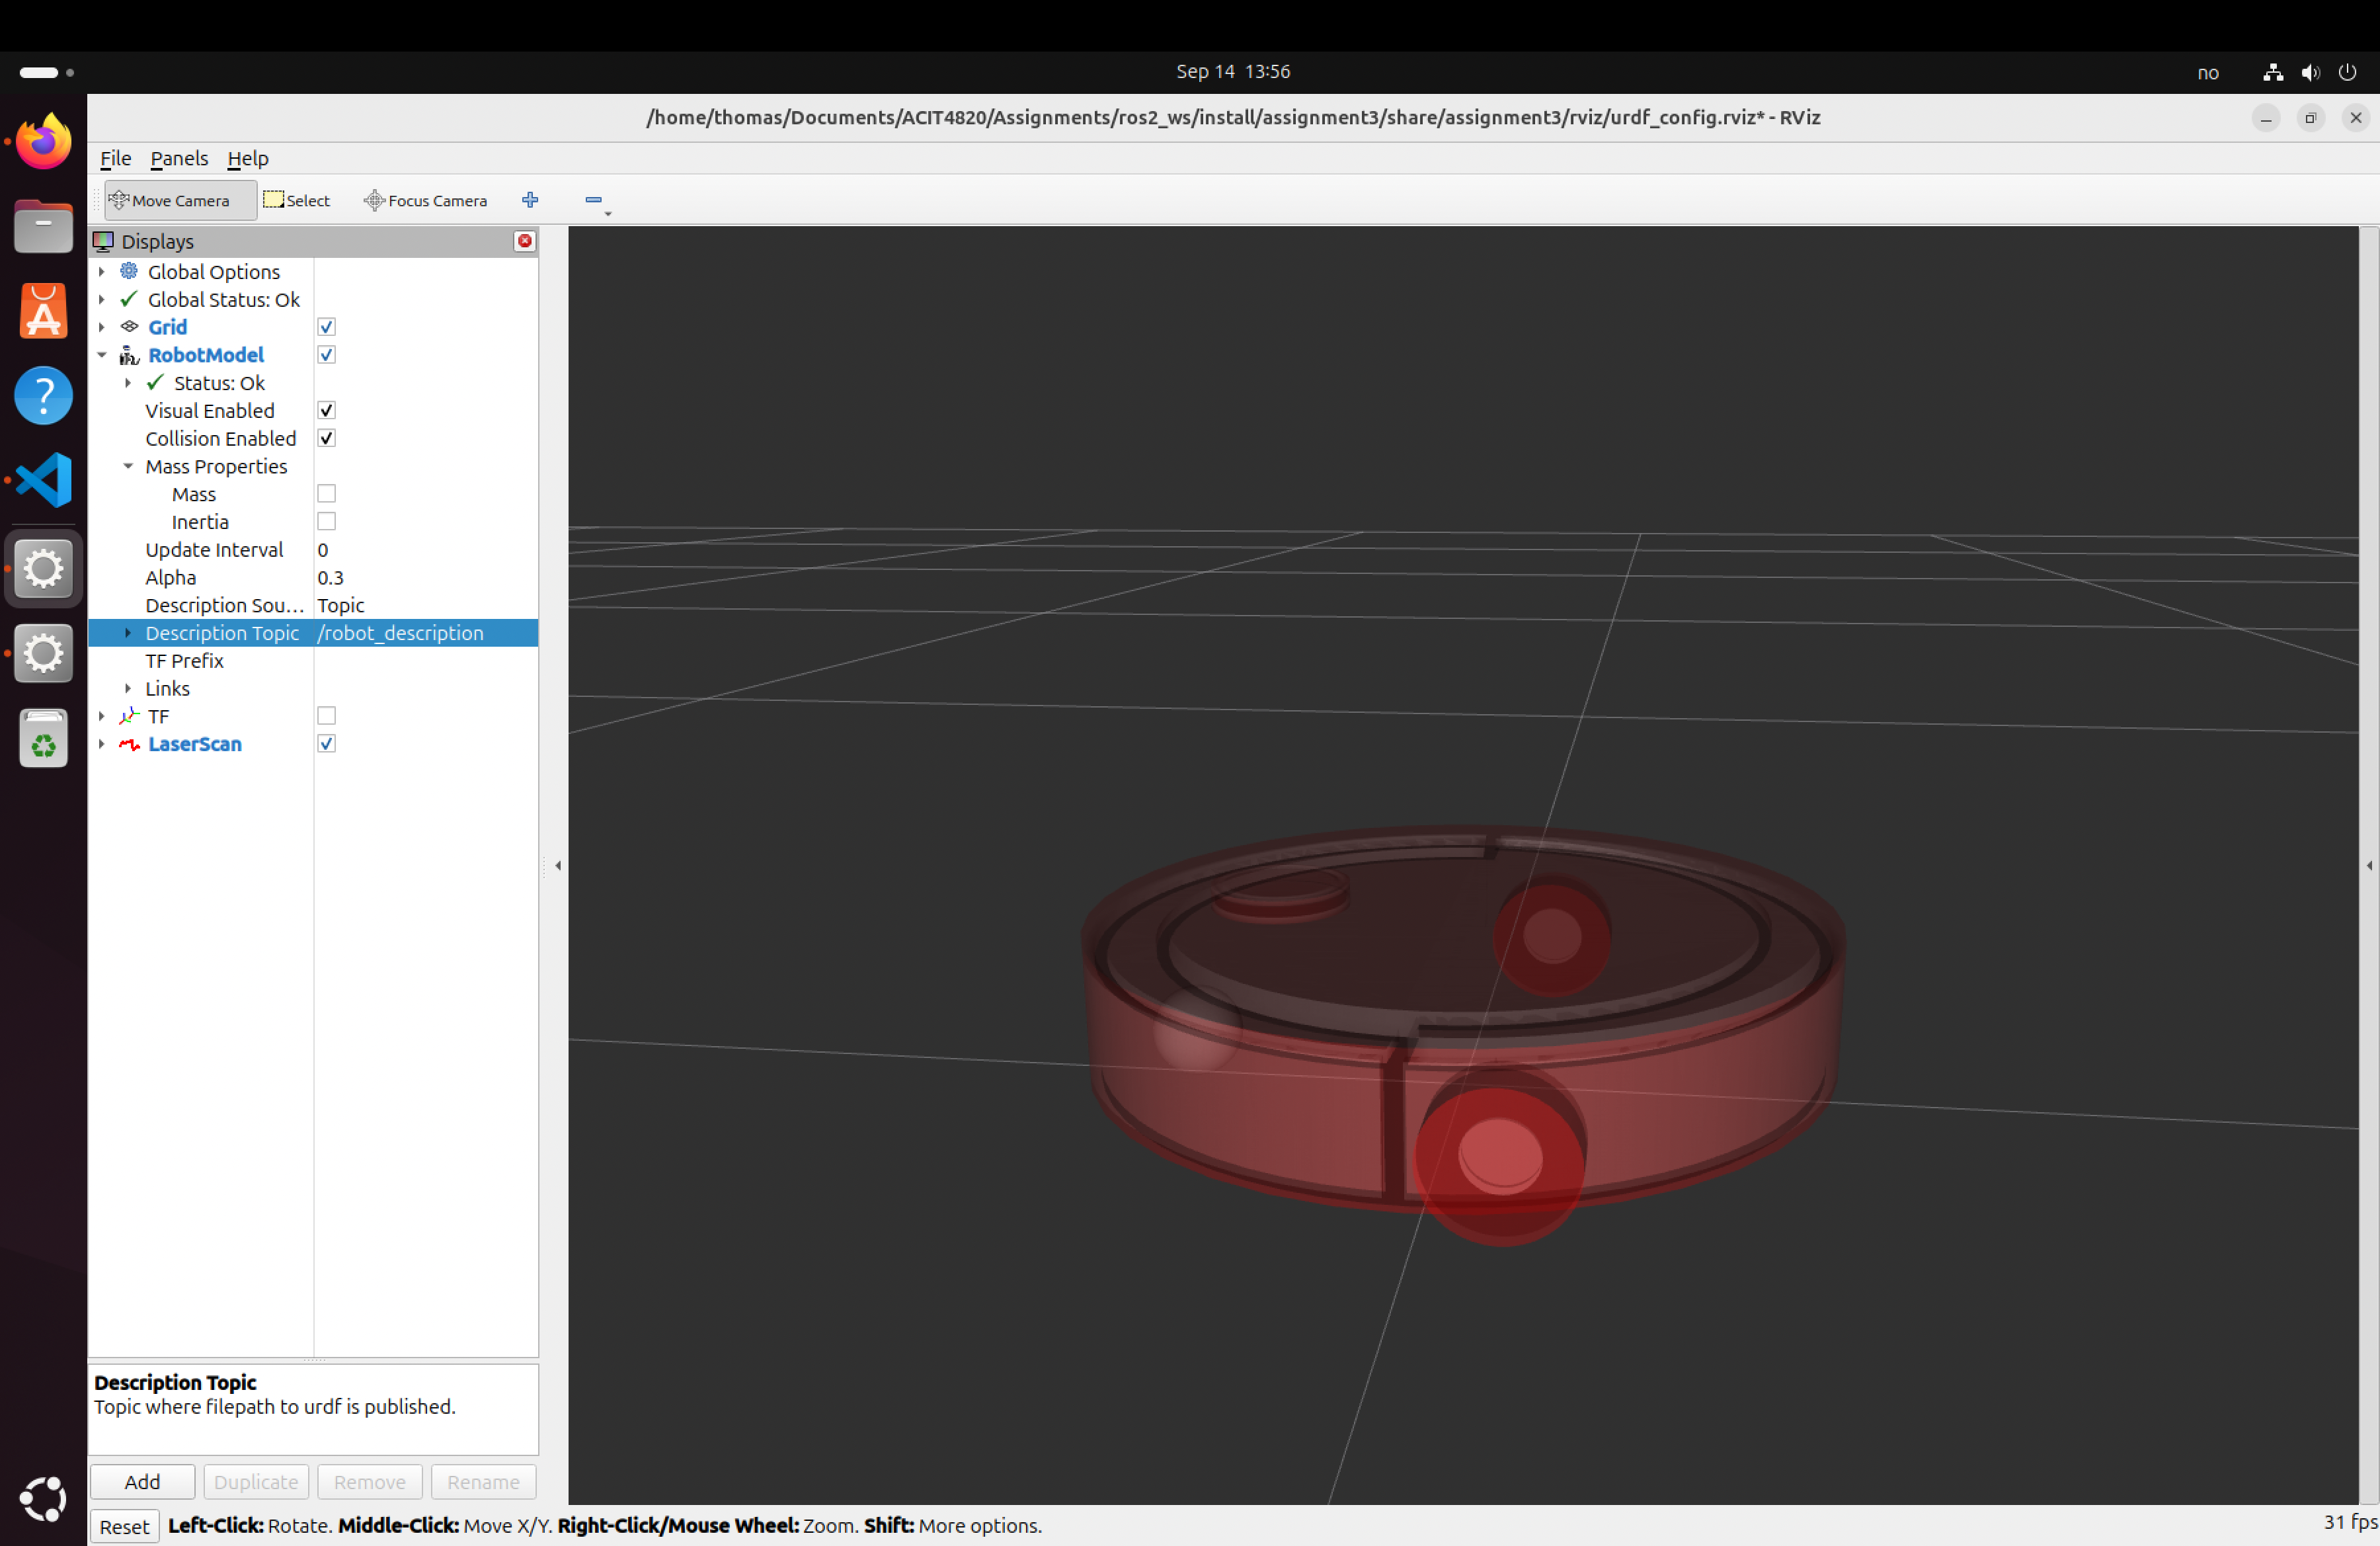
\includegraphics[width=\columnwidth]{fig/Task1/00_task1.png}
    \caption{Collision overlay in RViz. The Alpha is lowered so the collision
             primitives show through the meshes.}
    \label{fig:t1_collision}
\end{figure}

\section{Reflection}


\section{Use of AI}

\end{document}
